\documentclass[12pt]{article}
\usepackage[utf8]{inputenc}
\usepackage{graphicx}
\usepackage{float}
\usepackage{subcaption}
\usepackage[left=2cm, right=2cm, top=3cm]{geometry}

\renewcommand*\contentsname{Sumário}

\begin{document}

\begin{titlepage}
\begin{figure}[t]
\centering
\includegraphics[scale=0.6]{Images/ufpe2.png}
\label{fig_ufpe}
\end{figure}
\begin{center} 
{\large Luis Felipe Batista Pereira}\\[0.2cm]
{\large Marcos Heitor Carvalho de Oliveira}\\[0.2cm]
{\large Thalisson Moura Tavares}\\[5.5cm]
{\bf \Large RELATÓRIO DE PROJETO}\\[0.2cm]
{\large Métodos Numéricos}\\[5.5cm]
{\large Recife}\\[0.1cm]
{\large 2019}
\end{center}
\end{titlepage}

\tableofcontents
\newpage

\section{Introdução}
Visando compreender melhor os temas abordados em métodos numéricos abordamos quatro problemas direferentes indicados pelo professor \textbf{Ricardo Martins} dentro do conteúdo da cadeira de \textbf{Métodos Numéricos Computacionais} (if816ec) no CIN-UFPE.  




\section{Problema 1}

\subsection{Problema}
Durante a caçada pelas joias do infinito, após conseguir todas elas, Thanos dizimou metado do Universo. Sabe-se que a população de determinada cidade cresce a uma taxa propocional ao número de habitantes existentes. Se, após 10 anos do estalo de Thanos, a população triplica, e após 20 anos é de 150.000 habitantes, determine a população inicial.

\subsection{Modelo}
Ao vermos o Modelo de Crescimento Exponencial, isto é, a taxa de variação da população em relação ao tempo, aqui denotada por dP/dt, é proporcional à população presente. Em outras palavras, se P=P(t) mede a população, nós temos
\begin{equation}
    \frac{dP}{dt} = -k \cdot P(t)
\label{eq_1}
\end{equation}
onde a taxa k é uma constante.

\subsection{Solução Analítica}
Deseja-se obter a população inicial, logo a equação diferencial é da forma
\begin{equation}
    \frac{dP}{dt} = k \cdot P(t)
\label{eq_2}
\end{equation}
Como pode-se observar, a equação \ref{eq_2} é do tipo separável, logo a partir da equação \ref{eq_2} temos
\begin{equation}
    \frac{dP}{P(t)} = k \cdot dt
\end{equation}
Integrando ambos os lados da equação
\begin{equation}
    \int \frac{dP}{P(t)} = \int k \cdot\, dt
\label{eq_4}
\end{equation}
E resolvendo a integral
\begin{equation}
    \ln{P(t)} = kt + k_0
\label{eq_1_5}
\end{equation}
Da equação \ref{eq_1_5} obtemos
\begin{equation}
    e^{\ln{P(t)}} = e^{kt + k_0}
\label{eq_1_6}
\end{equation}
Sendo a solução geral da equação diferencial \ref{eq_2} igual a
\begin{equation}
    P(t) = k_0 \cdot e^{kt}
\label{eq_1_7}
\end{equation}
O problema informa que a população triplica em 10 anos, ou seja
\begin{equation}
    3 \cdot k_0 = k_0 \cdot e^{10k}
\label{eq_1_8}
\end{equation}
\begin{equation}
    3 = e^{10k}
\label{eq_1_9}
\end{equation}
Aplicando logaritmo natural de ambos os lados da equação \ref{eq_1_9} obtemos
\begin{equation}
    \ln{3} = \ln{e^{10k}}
\label{eq_1_10}
\end{equation}
Usando as regras de logaritmo
\begin{equation}
    10k = \ln{3}
\label{eq_1_11}
\end{equation}
\begin{equation}
    k = \frac{\ln{3}}{10}
\label{eq_1_12}
\end{equation}
Encontrando assim o valor da constante k
\begin{equation}
    k \approx 0,11
\label{eq_1_13}
\end{equation}
Substituindo o valor de k na equação \ref{eq_1_7} e usando o fato que P(20) = 150.000, obtemos
\begin{equation}
    150.000 = k_0 \cdot e^{0,11 \cdot 20}
\label{eq_1_14}
\end{equation}
logo 
\begin{equation}
    k_0 = \frac{150.000}{e^{0,11 \cdot 20}} \approx 16.620
\label{eq_1_14}
\end{equation}
Obtemos assim que a população inicial é de aproximadamente 16.620 habitantes e a solução geral do problema é
\begin{equation}
    P(t) = 16620 \cdot e^{0,11t}
\label{eq_1_14}
\end{equation}

\newpage


\subsection{Gráficos das Soluções Numéricas}
Nessa seção são apresentados os gráficos gerados pelos métodos numéricos implementados na parte 1 do projeto para a equação diferencial \ref{eq_1_14}

\begin{figure}[H]
\begin{subfigure}{.5\textwidth}
  \centering
  % include first image
  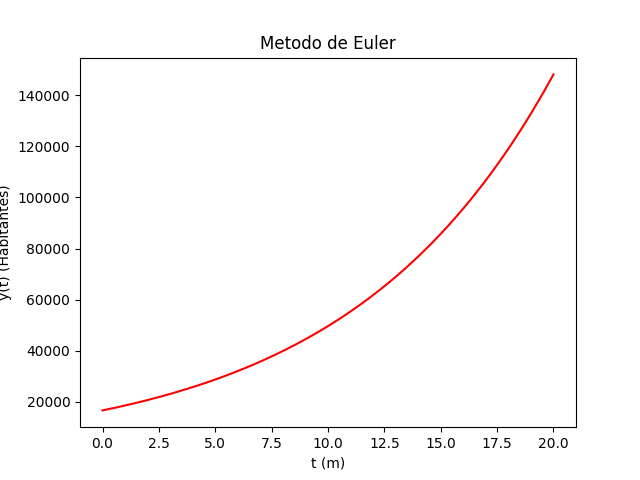
\includegraphics[width=.8\linewidth]{Images/q1/Euler_q1.png}  
  \caption{Euler}
\end{subfigure}
\begin{subfigure}{.5\textwidth}
  \centering
  % include second image
  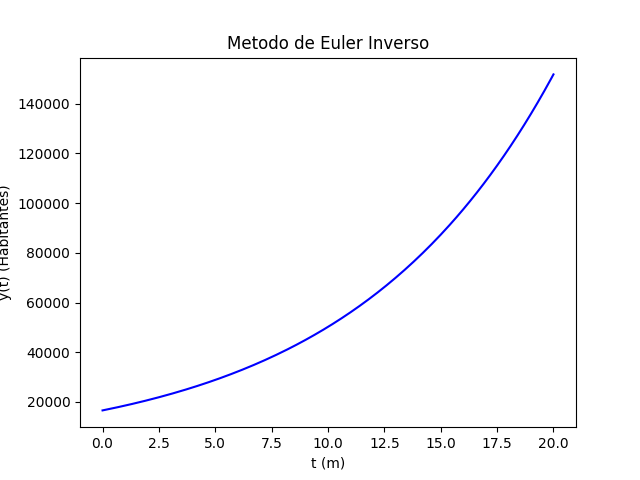
\includegraphics[width=.8\linewidth]{Images/q1/Euler_inv_q1.png}  
  \caption{Euler Inverso}
\end{subfigure}

\newline

\begin{subfigure}{.5\textwidth}
  \centering
  % include third image
  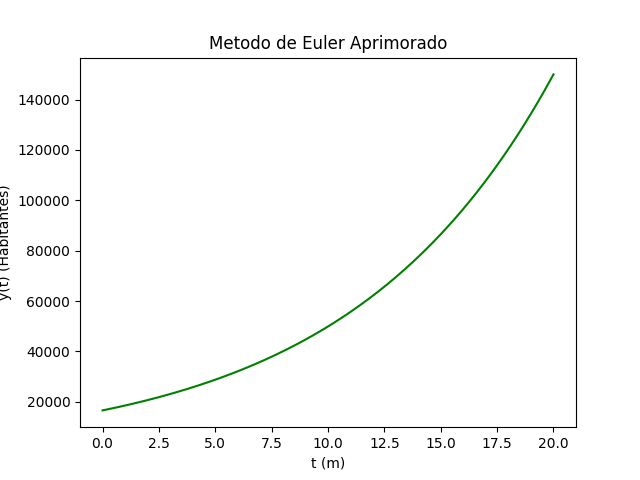
\includegraphics[width=.8\linewidth]{Images/q1/Euler_apr_q1.png}  
  \caption{Euler Aprimorado}
\end{subfigure}
\begin{subfigure}{.5\textwidth}
  \centering
  % include fourth image
  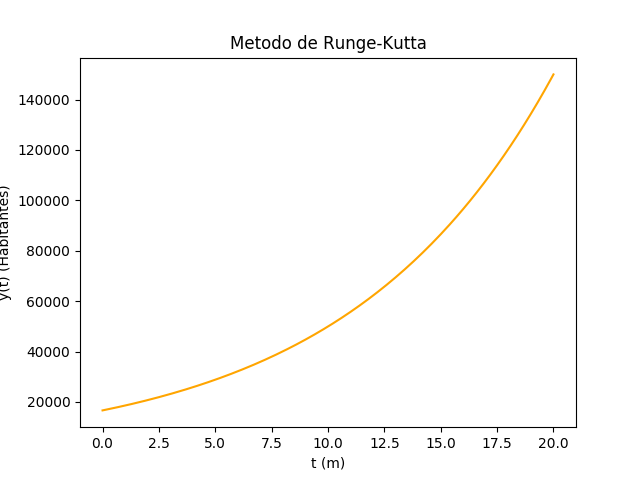
\includegraphics[width=.8\linewidth]{Images/q1/Runge_Kutta_q1.png}  
  \caption{Runge Kutta}
\end{subfigure}
\caption{Métodos de Passos simples}
\end{figure}

\begin{figure}[H]
\begin{subfigure}{.5\textwidth}
  \centering
  % include first image
  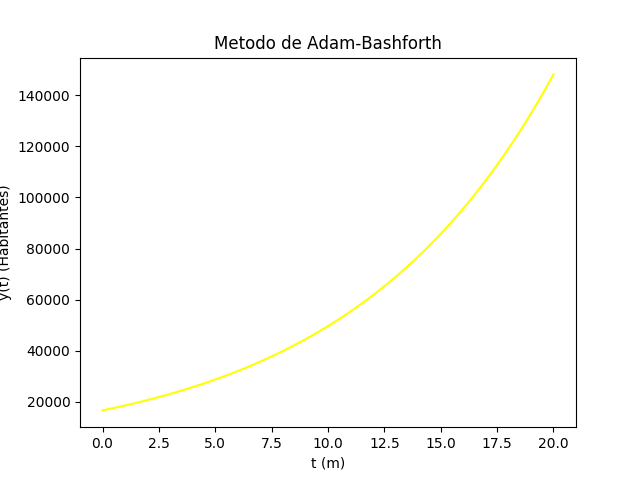
\includegraphics[width=.8\linewidth]{Images/q1/Adam_Bashforth_q1.png}  
  \caption{Adam Bashforth}
\end{subfigure}
\begin{subfigure}{.5\textwidth}
  \centering
  % include second image
  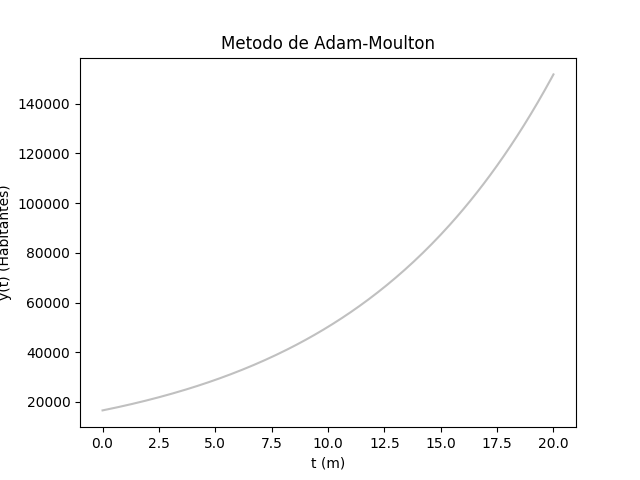
\includegraphics[width=.8\linewidth]{Images/q1/Adam_Moulton_q1.png}  
  \caption{Adam Moulton}
\end{subfigure}

\newline

\begin{subfigure}{.5\textwidth}
  \centering
  % include third image
  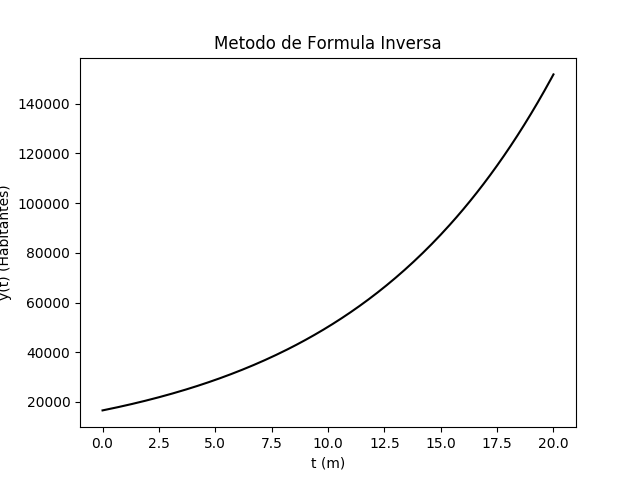
\includegraphics[width=.8\linewidth]{Images/q1/Formula_Inversa_q1.png}  
  \caption{Fórmula Inversa}
\end{subfigure}
\caption{Métodos de Passos Múltiplos}
\end{figure}

\subsection{Gráfico da Solução Analítica}
O gráfico da solução analítica é mostrado na figura abaixo

\begin{figure}[H]
\centering
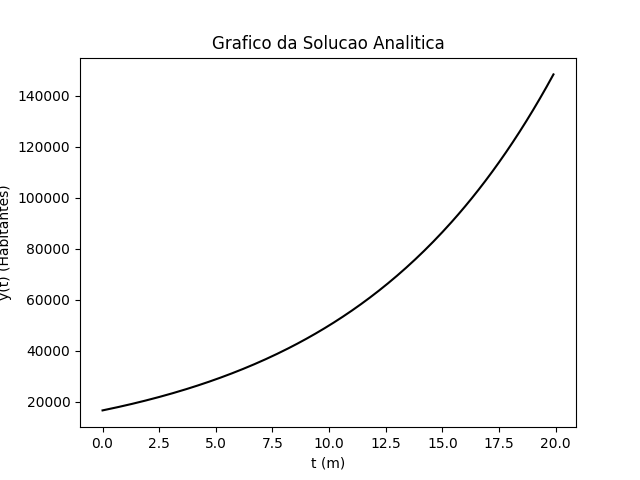
\includegraphics[scale=.5]{Images/q1/Analytic_solve_q1.png}
\label{fig_q1_SA}
\end{figure}

\subsection{Comparação e análise de desempenho}
Analisando a tabela dos métodos em conjunto com o erro associado podemos notar que tanto o método de Adam-Multon como o de Fórmula Inversa apresentam uma maior precisão em comparação aos outros para a solução real nesse caso.
\begin{figure}[H]
\centering
\includegraphics[width=\textwidth]{Images/q1_comp.png}
\label{fig_q1_comp}
\end{figure}





\section{Problema 2}

\subsection{Problema}
Um grande tanque de mistura contendo 300 galões de salmoura (isto é, água na qual foi dissolvida uma determinada quantidade de libras de sal) com 50 libras de sal. Outra salmoura é bombeada para dentro do tanque a uma taxa de três galões por minuto (3gal/min); a concentração de sal nessa segunda salmoura é de 2 libras por galão (2lbs/gal). Quando a solução no tanque estiver bem misturada, ela será bombeada para fora a mesma taxa em que a segunda salmoura entrou. Se A(t) denotar a quantidade de sal (medida em libras) no tanque no instante t, a taxa segundo a qual A(t) varia será uma taxa liquida. Determine a quantidade de sal no tanque em qualquer instante e calcule o instante de tempo, em minutos, para que A(t)=100.
\subsection{Modelo}
As variações na quantidade de sal são devidas somente aos fluxos de entrada e de saida do tanque. Mais precisamente a taxa de variação de sal no tanque, dA/dt, é igual a taxa segundo a qual o sal está entrando menos a taxa segundo a qual ele está saindo
\begin{equation}
    \frac{dA}{dt} = entrada - saida
\end{equation}
A taxa de entrada de sal no tanque é a concentração 2 lbs/gal vezes a taxa de fluxo 3 gal/min.
\begin{equation}
    entrada = 3 \frac{gal}{min} \cdot 2 \frac{lbs}{gal}
\end{equation}
\begin{equation}
    entrada = 6 \frac{lbs}{min}
\end{equation}
Para encontrar a taxa segundo a qual o sal deixa o tanque precisamos multiplicar a concentração de sal no tanque pela taxa de fluxo, 3 gal/min. Como as taxas de fluxo de saída e de entrada são iguais, o volume de água no tanque permanece constante e igual a 300gal; como a mistura está "bem mexida", a concentração é uniforme no tanque, A(t)/300 lbs/gal. Portanto, a taxa de saída do sal no tanque é
\begin{equation}
    saida = 3 \cdot \frac{A(t)}{300}
\end{equation}
\begin{equation}
    saida = \frac{A(t)}{100}
\end{equation}
Logo, a equação diferencial que governa esse processo é
\begin{equation}
    \frac{dA}{dt} = 6 - \frac{A(t)}{100}
\label{eq_7}
\end{equation}

\subsection{Solução Analítica}
A primeira parte do problema pede a solução geral da equação diferencial \ref{eq_7}, a partir dela temos
\begin{equation}
    \frac{dA}{dt} + \frac{A(t)}{100} = 6 
\label{eq_8}
\end{equation}
Resolvendo a equação pelo método do fator integrante, temos que o fator integrante é
\begin{equation}
    \mu(t) = e^{t/100}
\end{equation}
Multiplicando a equacão diferencial \ref{eq_8} pelo fator integrante, obtemos
\begin{equation}
    \frac{dA}{dt} \cdot e^{t/100} + e^{t/100}\cdot \frac{A(t)}{100} = 6 \cdot e^{t/100}
\end{equation}
ou
\begin{equation}
    \frac{d}{dt}(e^{t/100}\cdot A(t)) = 6 \cdot e^{t/100}
\label{eq_11}
\end{equation}
Integrando a equação diferencial, temos
\begin{equation}
    e^{t/100}\cdot A(t) = \int_{}^{} 6 \cdot e^{t/100}\, dt
\end{equation}
\begin{equation}
    e^{t/100}\cdot A(t) = 600 \cdot e^{t/100} + c
\end{equation}
onde c é uma constante arbitrária, logo obtemos
\begin{equation}
    A(t) = 600 + c \cdot e^{-t/100}
\label{eq_14}
\end{equation}
A partir da descrição do problema verificamos que a quantidade inicial de sal é de 50 libras
\begin{equation}
    A(0) = 50
\end{equation}
Sendo assim, substituindo os valores no instante de tempo t=0 na equação \ref{eq_14} temos
\begin{equation}
    A(0) = 600 + c \cdot e^{-0/100}
\end{equation}
ou
\begin{equation}
    50 = 600 + c
\end{equation}
Resultando
\begin{equation}
    c = -550
\end{equation}
Logo, a solução geral da \ref{eq_8} é
\begin{equation}
    A(t) = 600 - 550 \cdot e^{-t/100}
\label{eq_19}
\end{equation}
A partir da solução geral resolvemos a segunda parte do problema, a qual deseja-se obter o instante de tempo, em minutos, para o qual a quantidade de sal é igual a 100 libras. Substituindo os valores na equação \ref{eq_19}
\begin{equation}
    100 = 600 - 550 \cdot e^{-t/100}
\end{equation}
ou
\begin{equation}
    500 = 550 \cdot e^{-t/100}
\end{equation}
segue que
\begin{equation}
    e^{-t/100} = \frac{500}{550}
\label{eq_22}
\end{equation}
Aplicando logaritmo natural de ambos os lados da equação \ref{eq_22}
\begin{equation}
    \ln{e^{-t/100}} = \ln{\frac{500}{550}}
\end{equation}
assim, usando as regras de logaritmo obtemos
\begin{equation}
    -\frac{t}{100} = \ln{\frac{500}{550}}
\end{equation}
ou
\begin{equation}
    {t} = -\ln{\frac{500}{550}} \cdot 100 \approx 9,53min
\end{equation}
Logo o instante de tempo para o qual a quantidade de sal no tanque seja igual a 100 libras é aproximadamente 9,53 minutos.
\subsection{Gráficos das Soluções Numéricas}
Nessa seção são apresentados os gráficos gerados pelos métodos numéricos implementados na parte 1 do projeto para a equação diferencial \ref{eq_7}
\begin{figure}[H]
\begin{subfigure}{.5\textwidth}
  \centering
  % include first image
  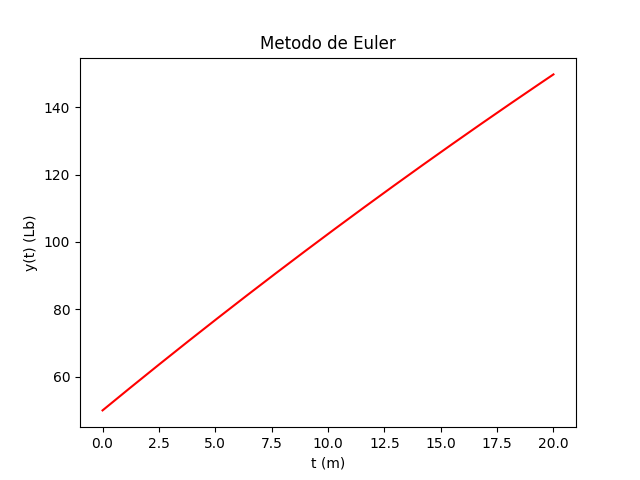
\includegraphics[width=.8\linewidth]{Images/q2/Euler_q2.png}  
  \caption{Euler}
\end{subfigure}
\begin{subfigure}{.5\textwidth}
  \centering
  % include second image
  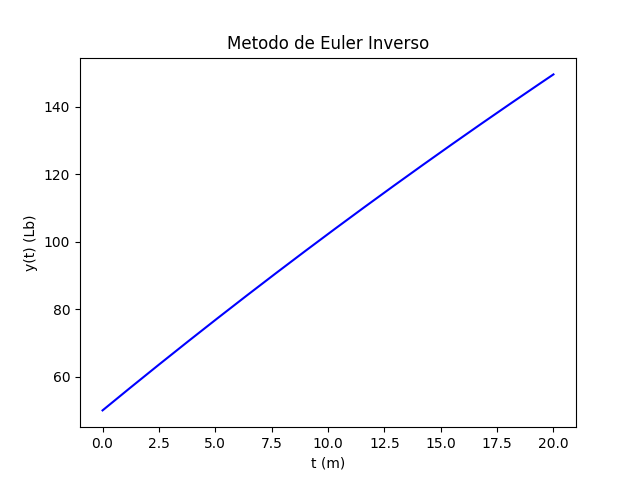
\includegraphics[width=.8\linewidth]{Images/q2/Euler_inv_q2.png}  
  \caption{Euler Inverso}
\end{subfigure}

\newline

\begin{subfigure}{.5\textwidth}
  \centering
  % include third image
  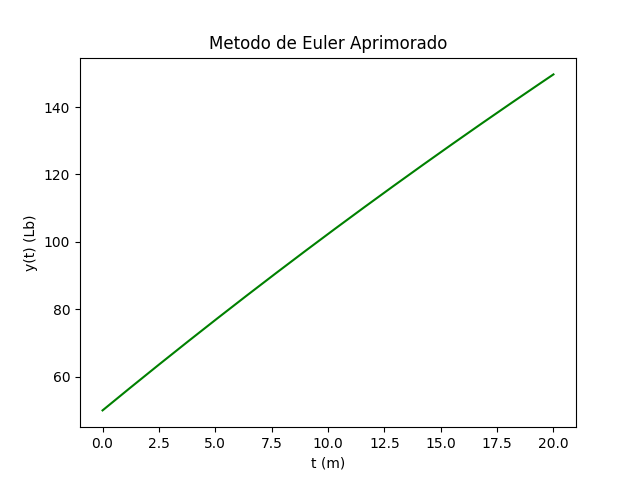
\includegraphics[width=.8\linewidth]{Images/q2/Euler_apr_q2.png}  
  \caption{Euler Aprimorado}
\end{subfigure}
\begin{subfigure}{.5\textwidth}
  \centering
  % include fourth image
  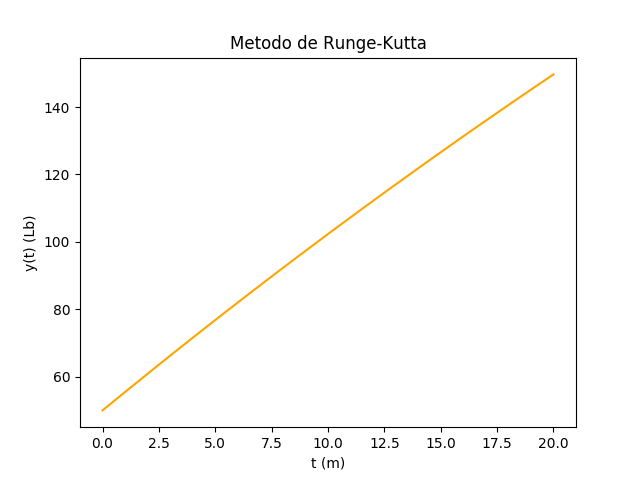
\includegraphics[width=.8\linewidth]{Images/q2/Runge_Kutta_q2.png}  
  \caption{Runge Kutta}
\end{subfigure}
\caption{Métodos de Passos simples}
\end{figure}

\begin{figure}[H]
\begin{subfigure}{.5\textwidth}
  \centering
  % include first image
  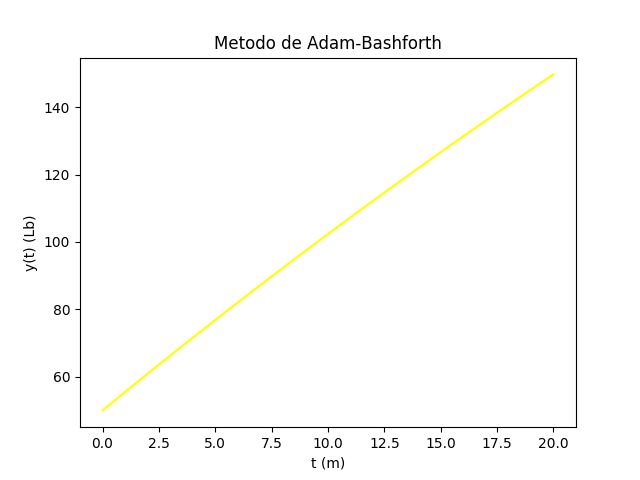
\includegraphics[width=.8\linewidth]{Images/q2/Adam_Bashforth_q2.png}  
  \caption{Adam Bashforth}
\end{subfigure}
\begin{subfigure}{.5\textwidth}
  \centering
  % include second image
  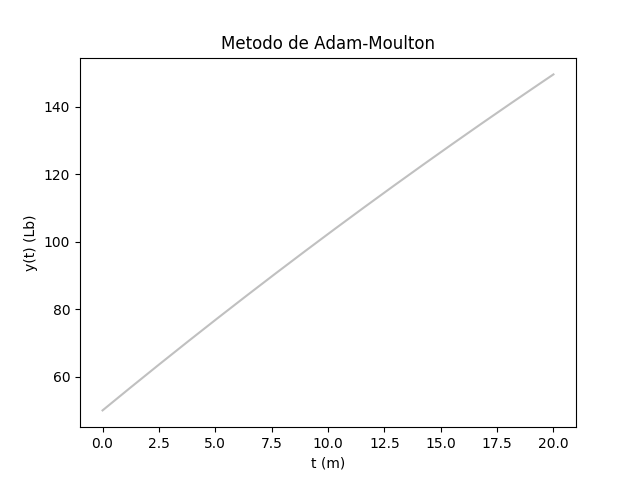
\includegraphics[width=.8\linewidth]{Images/q2/Adam_Moulton_q2.png}  
  \caption{Adam Moulton}
\end{subfigure}

\newline

\begin{subfigure}{.5\textwidth}
  \centering
  % include third image
  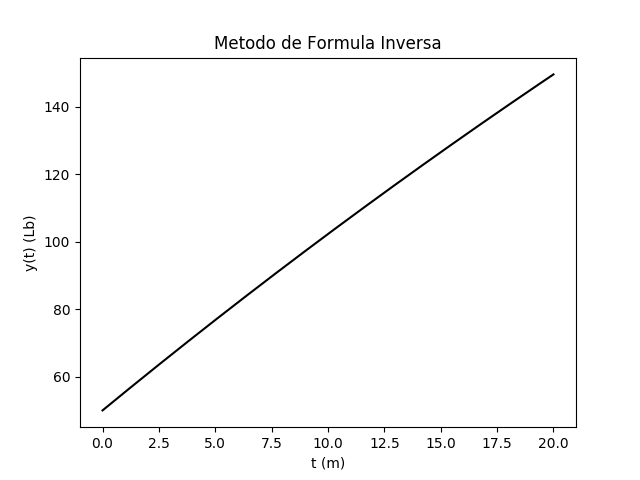
\includegraphics[width=.8\linewidth]{Images/q2/Formula_Inversa_q2.png}  
  \caption{Formula Inversa}
\end{subfigure}
\caption{Métodos de Passos Múltiplos}
\end{figure}

\subsection{Gráfico da Solução Analítica}
O gráfico da solução analítica é mostrado na figura abaixo

\begin{figure}[H]
\centering
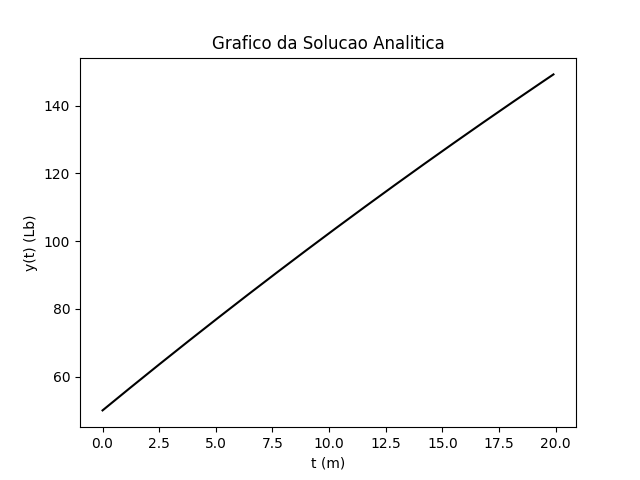
\includegraphics[scale=.5]{Images/q2/Analytic_solve_q2.png}
\label{fig_q2_SA}
\end{figure}
\subsection{Comparação e análise de desempenho}
Analisando a tabela dos métodos em conjunto com o erro associado podemos notar que tanto o método de Euler como o de Adams-Bashforth apresentam uma maior precisão em comparação aos outros para a solução real nesse caso.
\begin{figure}[H]
\centering
\includegraphics[width=\textwidth]{Images/q2_comp.png}
\label{fig_q2_comp}
\end{figure}




\section{Problema 3}

\subsection{Problema}
Um bolo é retirado do forno, sua temperatura é de 300ºF. Três minutos depois, sua temperatura passa para 200ºF. Quanto tempo levará para sua temperatura chegar a 75 graus, se a temperatura do meio ambiente em que ele foi colocado for de exatamente 70ºF?
\subsection{Modelo}
De acordo com a Lei empírica de Newton do esfriamento/resfriamento, a taxa segundo a qual a temperatura de um corpo varia é proporcional a diferença entre a temperatura do corpo e a temperatura do meio em que rodeia, denominada temperatura ambiente. Se T(t) representar a temperatura do corpo no instante t, Tm a temperatura do meio que o rodeia dT/dt a taxa segundo a qual a temperatura do corpo varia, a lei de Newton do esfriamento/resfriamento é convertido na sentença matemática
\begin{equation}
    \frac{dT}{dt} = k(T-T_m)
\label{eq_3_41}
\end{equation}
\begin{equation}
    T = ce^{kt}+T_m
\label{eq_3_42}
\end{equation}
onde k é uma constante de proporcionalidade. Em ambos os casos, esfriamento ou aquecimento, se Tm for uma constatne, é lógico que k é menor que 0.
\subsection{Solução Analítica}
Queremos saber o tempo t, tal que T(t) = 75ºF, tendo em vista a equação diferencial \ref{eq_3_41} e sua solução na equação \ref{eq_3_42}, temos que encontrar os valores das constantes c e k. O enunciado do problema informa que no instante t=0 a temperatura é igual a 300ºF e que a temperatura do meio é igual a 70ºF, obtemos assim
\begin{equation}
    300 = ce^{0}+70
\label{eq_3_43}
\end{equation}
onde
\begin{equation}
    c = 300-70 = 230
\label{eq_3_44}
\end{equation}
Quando t=3 a temperatura é igual a 200ºF, substituindo na equação \ref{eq_3_42} os respectivos valores
\begin{equation}
    200 = 230 \cdot e^{3k}+70
\label{eq_3_45}
\end{equation}
\begin{equation}
    130 = 230 \cdot e^{3k}
\label{eq_3_46}
\end{equation}
Aplicando ln de ambos os lados da equação
\begin{equation}
    \ln{23e^{3k}} = \ln{13}
\label{eq_3_47}
\end{equation}
Após aplicar regras de logaritmo obtemos
\begin{equation}
    \ln{23}+3k \cdot \ln{e} = \ln{13}
\label{eq_3_48}
\end{equation}
logo temos que a constante k é
\begin{equation}
    k = \frac{\ln{13} - \ln{23}}{3} \approx -0,19
\label{eq_3_49}
\end{equation}
O que faz sentido a constante k ser nagativa para o sistema proposto. Substituindo os valores encontrados na equação \ref{eq_3_42}
\begin{equation}
    T(t) = 230 \cdot e^{-0,19t} + 70
\label{eq_3_50}
\end{equation}
Deseja-se encontrar o instante para o qual a temperatura é igual a 75ºF, logo da equação \ref{eq_3_50} temos
\begin{equation}
    75 = 230 \cdot e^{-0,19t} + 70
\label{eq_3_51}
\end{equation}
\begin{equation}
    230 \cdot e^{-0,19t} = 5
\label{eq_3_52}
\end{equation}
aplicando ln de ambos os lados da equação 
\begin{equation}
    \ln{230e^{-0,19t}} = \ln{5}
\label{eq_3_53}
\end{equation}
e usando regras de logaritmo, obtemos
\begin{equation}
    \ln{230} - 0,19t = \ln{5}
\label{eq_3_54}
\end{equation}
Assim, o instante t para o qual a temperatura é 75ºF é
\begin{equation}
    t = -\frac{\ln{5} - \ln{230}}{0,19} \approx 20,13min
\end{equation}{}

\subsection{Gráficos das Soluções Numéricas}

Nessa seção são apresentados os gráficos gerados pelos métodos numéricos implementados na parte 1 do projeto para a equação diferencial \ref{eq_3_50}
\begin{figure}[H]
\begin{subfigure}{.5\textwidth}
  \centering
  % include first image
  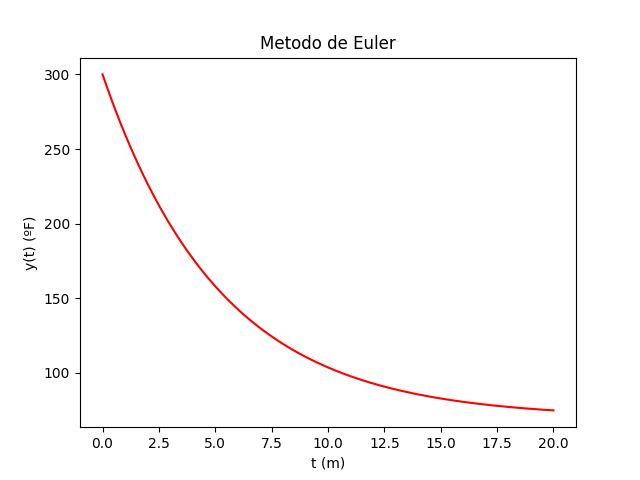
\includegraphics[width=.8\linewidth]{Images/q3/Euler_q3.png}  
  \caption{Euler}
\end{subfigure}
\begin{subfigure}{.5\textwidth}
  \centering
  % include second image
  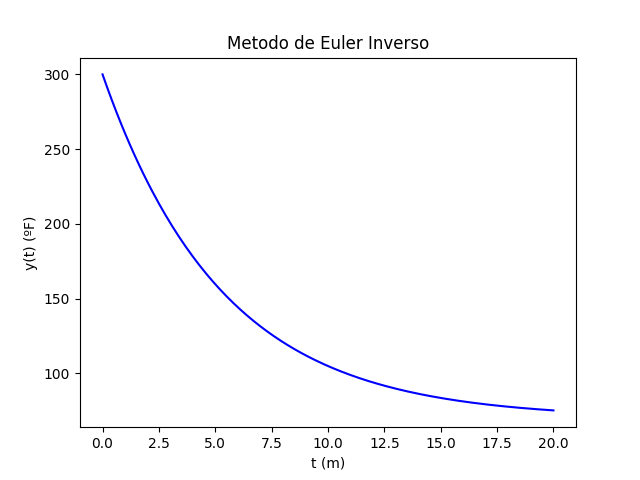
\includegraphics[width=.8\linewidth]{Images/q3/Euler_inv_q3.png}  
  \caption{Euler Inverso}
\end{subfigure}

\newline

\begin{subfigure}{.5\textwidth}
  \centering
  % include third image
  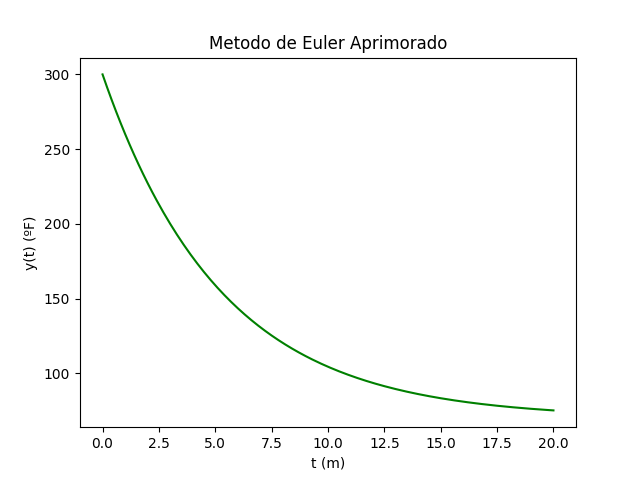
\includegraphics[width=.8\linewidth]{Images/q3/Euler_apr_q3.png}  
  \caption{Euler Aprimorado}
\end{subfigure}
\begin{subfigure}{.5\textwidth}
  \centering
  % include fourth image
  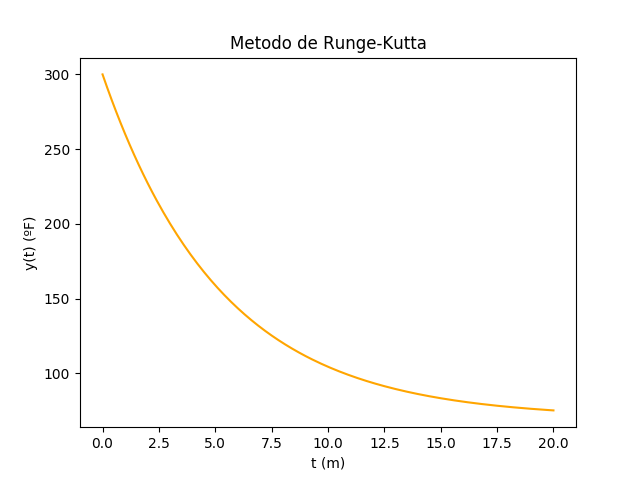
\includegraphics[width=.8\linewidth]{Images/q3/Runge_Kutta_q3.png}  
  \caption{Runge Kutta}
\end{subfigure}
\caption{Métodos de Passos simples}
\end{figure}

\begin{figure}[H]
\begin{subfigure}{.5\textwidth}
  \centering
  % include first image
  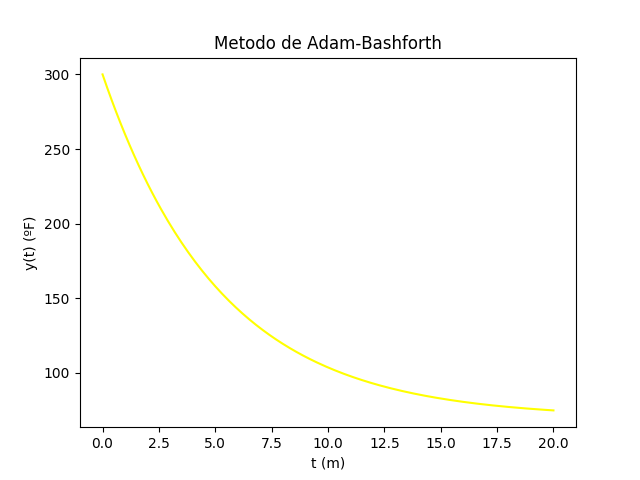
\includegraphics[width=.8\linewidth]{Images/q3/Adam_Bashforth_q3.png}  
  \caption{Adam Bashforth}
\end{subfigure}
\begin{subfigure}{.5\textwidth}
  \centering
  % include second image
  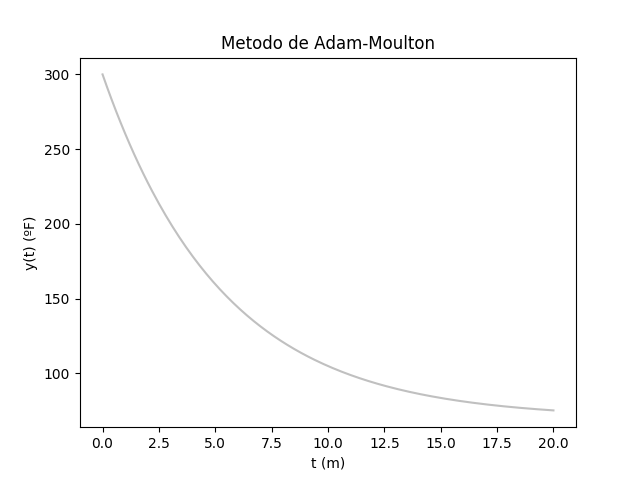
\includegraphics[width=.8\linewidth]{Images/q3/Adam_Moulton_q3.png}  
  \caption{Adam Moulton}
\end{subfigure}

\newline

\begin{subfigure}{.5\textwidth}
  \centering
  % include third image
  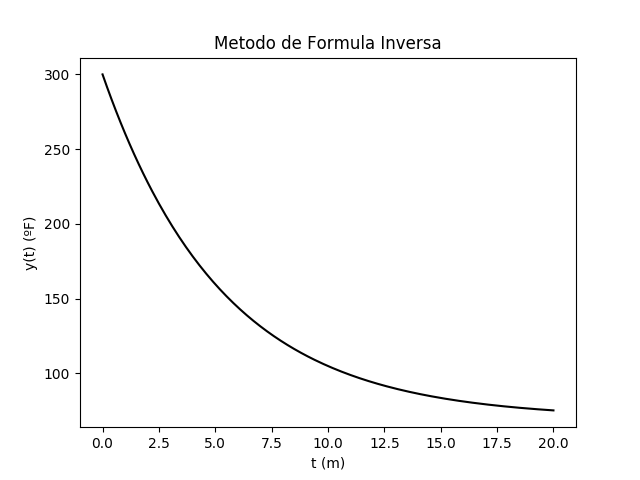
\includegraphics[width=.8\linewidth]{Images/q3/Formula_Inversa_q3.png}  
  \caption{Formula Inversa}
\end{subfigure}
\caption{Métodos de Passos Múltiplos}
\end{figure}

\subsection{Gráfico da Solução Analítica}
O gráfico da solução analítica é mostrado na figura abaixo

\begin{figure}[H]
\centering
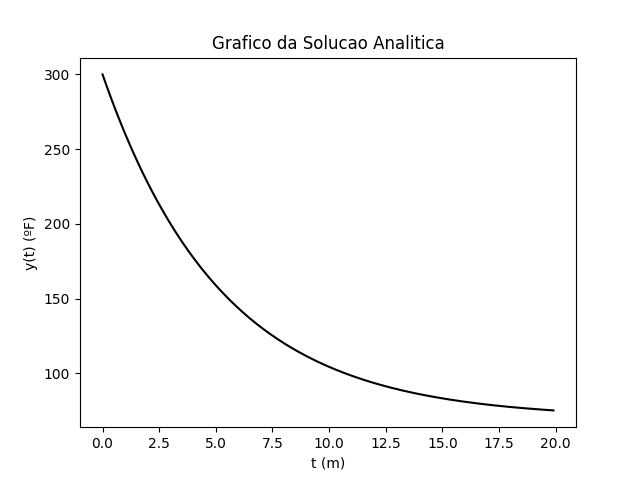
\includegraphics[scale=.5]{Images/q3/Analytic_solve_q3.png}
\label{fig_q3_SA}
\end{figure}
\subsection{Comparação e análise de desempenho}
Analisando a tabela dos métodos em conjunto com o erro associado podemos notar que tanto o método de Euler como o de Adams-Bashforth apresentam uma maior precisão em comparação aos outros para a solução real nesse caso.
\begin{figure}[H]
\centering
\includegraphics[width=\textwidth]{Images/q3_comp.png}
\label{fig_q3_comp}
\end{figure}




\section{Problema 4}

\subsection{Problema}
Descreva o sistema de equações diferenciais que descreve i1(t) e i2(t) no circuito eletrico contendo um registor , um indutor e um capacitor mostrado na figura \ref{fig_4a}, e resolva por laplace o sistema encontrado supondo que E(t)=60, L=1H, R=50Ohm e $C=10^{-4}$F e que inicialmente i1=i2=0 (ver figura \ref{fig_4b})  
\begin{figure}[H]
\centering
\includegraphics[scale=.6]{Images/4a.png}
\caption{Problema 4}
\label{fig_4a}
\end{figure}
\begin{figure}[H]
\centering
\includegraphics[scale=.6]{Images/4b.png}
\caption{Problema 4}
\label{fig_4b}
\end{figure}

\subsection{Modelo}
A lei das malhas diz que a soma das diferenças de potenciais em uma malha é igual a zero, logo a partir da malha esquerda da figura \ref{fig_4a} temos
\begin{equation}
    E - L \frac{di_1}{dt} - i_2R = 0
\label{eq_4_56}
\end{equation}
Da malha direita da figura \ref{fig_4a} obtemos
\begin{equation}
    \frac{1}{C} \int_{0}^{t} i_3\,dt - i_2R = 0
\label{eq_4_57}
\end{equation}
Resolvendo a integral da equação \ref{eq_4_57}
\begin{equation}
    \frac{i_3t}{C} - i_2R = 0
\label{eq_4_58}
\end{equation}
E derivando a equação \ref{eq_4_58} em relação ao tempo
\begin{equation}
    \frac{i_3}{C} - \frac{di_2}{dt}R = 0
\label{eq_4_59}
\end{equation}
Pela regra da conservação das cargas sabemos que 
\begin{equation}
    i_1 = i_2 + i_3
\label{eq_4_60}
\end{equation}
substituindo o valor de $i_3$ na equação \ref{eq_4_59} ficamos com
\begin{equation}
    \frac{i_1-i_2}{C} - \frac{di_2}{dt}R = 0
\label{eq_4_61}
\end{equation}
E por fim, multiplicando a equação \ref{eq_4_61} por C obtemos a seguinte equação
\begin{equation}
    i_1-i_2 - RC\frac{di_2}{dt} = 0
\label{eq_4_62}
\end{equation}
Temos então o sistema de equações formado pela equação \ref{eq_4_56} e pela equação \ref{eq_4_62} como a modelagem do problema 

\subsection{Solução Analítica}
Substituindo os valores informados no enunciado do problema nas equações \ref{eq_4_56} e \ref{eq_4_62} temos
\begin{equation}
    60 - \frac{di_1}{dt} - 50i_2 = 0
\label{eq_4_63}
\end{equation}
e
\begin{equation}
   i_1-i_2 - 5 \cdot 10^{-3}\frac{di_2}{dt} = 0
\label{eq_4_64}
\end{equation}
Aplicando laplace na equação \ref{eq_4_63} obtemos
\begin{equation}
   \mathcal{L}{\frac{di_1}{dt}} = 60 \cdot \mathcal{L}{1}-50\cdot \mathcal{L}{i_2}
\label{eq_4_65}
\end{equation}
Usando as transformadas de laplace, a equação \ref{eq_4_65} fica 
\begin{equation}
  s\cdot I_1-i_1(0)=\frac{60}{s}-50I_2
\label{eq_4_66}
\end{equation}
logo
\begin{equation}
   I_1 = \frac{60}{s^2}-\frac{50I_2}{s} 
\label{eq_4_67}
\end{equation}
Aplicando laplace na equação \ref{eq_4_64} temos

\begin{equation}
  \mathcal{L}{i_1} = \mathcal{L}{i_2} + 5 \cdot 10^{-3} \cdot \mathcal{L}{\frac{di_2}{dt}}
\label{eq_4_68}
\end{equation}

Usando as transformadas de laplace a equação \ref{eq_4_68} fica
\begin{equation}
  I_1 = I_2 \cdot (1+5\cdot 10^{-3}s)
\label{eq_4_69}
\end{equation}

Substituindo a equação \ref{eq_4_69} na equação \ref{eq_4_67} temos
\begin{equation}
  I_2 \cdot (1 + 5 \cdot 10^{-3}s + \frac{50}{s}) = \frac{60}{s^2}
\label{eq_4_70}
\end{equation}

Multiplicando ambos os lados da equação por s
\begin{equation}
    I_2 \cdot (s + 5 \cdot 10^{-3}s^2 + 50s) = \frac{60}{s}
\label{eq_4_71}
\end{equation}


Manipulando a equação \ref{eq_4_71} algebricamente
\begin{equation}
  I_2 = \frac{120}{s\cdot(s^2+2s+100)}
\label{eq_4_72}
\end{equation}

\begin{equation}
    I_2 = \frac{120}{s\cdot10^{-2}\cdot(s^2+2s+100)}
\label{eq_4_73}
\end{equation}


\begin{equation}
    I_2 = \frac{12000}{s\cdot(s+100)^2}
\label{eq_4_74}
\end{equation}

Usando a inversa de laplace na equação \ref{eq_4_74}
\begin{equation}
  i_2(t) = 12\cdot10^3 \int_{0}^{t} \tau e^{-100\tau}\,d\tau
\label{eq_4_75}
\end{equation}



E resolvendo a integral, encontramos o valor para $i_2$, segue
\begin{equation}
  i_2(t) = [\frac{1}{10000} - \frac{(100t+1)e^{-100t}}{10000}]\cdot 12 \cdot 10^3
\label{eq_4_76}
\end{equation}




\begin{equation}
  i_2(t) = -120te^{-100t}-1,2e^{-100t}+1,2
\label{eq_4_77}
\end{equation}



Substituindo a equação \ref{eq_4_74} na equação \ref{eq_4_69}, vemos que $I_1$ é 
\begin{equation}
  I_1 = \frac{12 \cdot 10^3}{s \cdot(s+100)^2} + \frac{60}{(s+100)^2}
\label{eq_4_78}
\end{equation}




Aplicando a inversa de laplace na equação \ref{eq_4_78} e substituindo o valor de $i_2$ encontrado na equação \ref{eq_4_77}, obtemos
\begin{equation}
  i_1 = -120te^{-100t} - 1,2e^{-100t} + 1,2 + 60te^{-100t}
\label{eq_4_79}
\end{equation}




segue que
\begin{equation}
  i_1 = -60te^{-100t}-1,2e^{-100t} +1,2
\label{eq_4_80}
\end{equation}
Logo a solução por laplace para o sistema encontrado na seção anterior e utilizando os valores informados no enunciado do problema é mostrada nas equações \ref{eq_4_77} e \ref{eq_4_80}.




\subsection{Gráficos das Soluções Numéricas}
Nessa seção são apresentados os gráficos gerados pelos métodos numéricos implementados na parte 1 do projeto para a corrente $i_1$, para a corrente $i_2$ a ideia é a mesma. 

\newline

\textbf{Observação:} para utilizar o método numérico foi necessário substituir uma solução analítica dentro da equação diferencial \ref{eq_4_63}, onde substituimos $i_2$ pelo valor dado na equação \ref{eq_4_77}, de forma que tivessemos uma equação diferencial ordinária simples. 

\begin{figure}[H]
\begin{subfigure}{.5\textwidth}
  \centering
  % include first image
  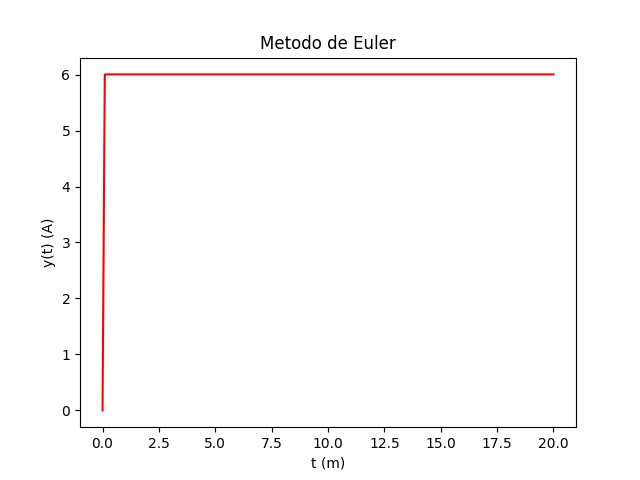
\includegraphics[width=.8\linewidth]{Images/q4/Euler_i1_q4.png}  
  \caption{Euler}
\end{subfigure}
\begin{subfigure}{.5\textwidth}
  \centering
  % include second image
  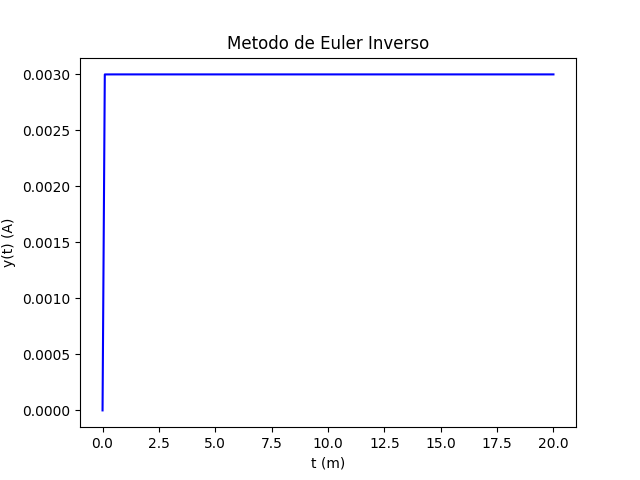
\includegraphics[width=.8\linewidth]{Images/q4/Euler_inv_i1_q4.png}  
  \caption{Euler Inverso}
\end{subfigure}

\newline

\begin{subfigure}{.5\textwidth}
  \centering
  % include third image
  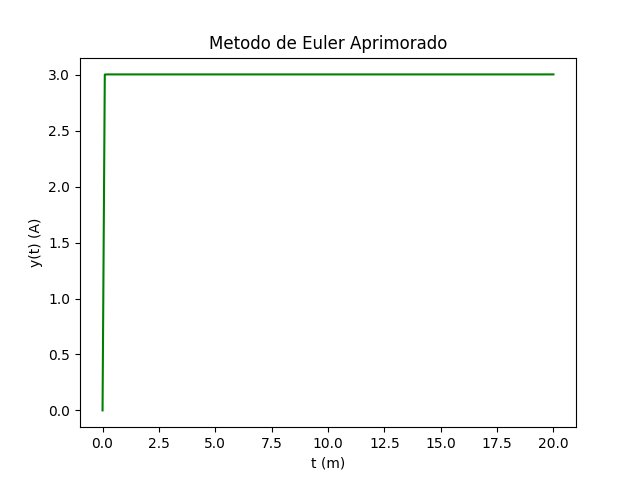
\includegraphics[width=.8\linewidth]{Images/q4/Euler_apr_i1_q4.png}  
  \caption{Euler Aprimorado}
\end{subfigure}
\begin{subfigure}{.5\textwidth}
  \centering
  % include fourth image
  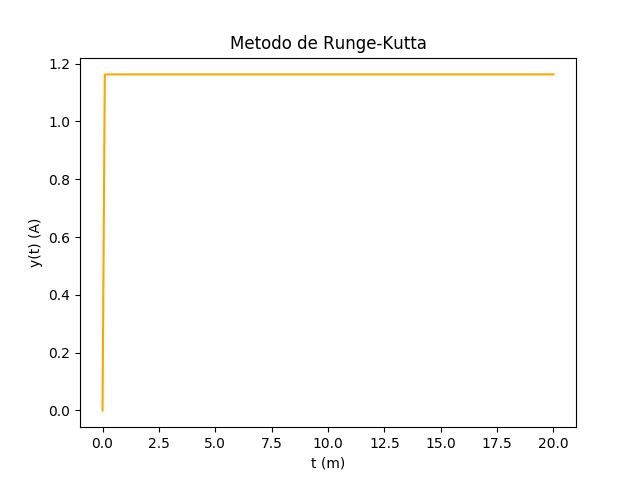
\includegraphics[width=.8\linewidth]{Images/q4/Runge-Kutta_i1_q4.png}  
  \caption{Runge Kutta}
\end{subfigure}
\caption{Métodos de Passos simples}
\end{figure}

\begin{figure}[H]
\begin{subfigure}{.5\textwidth}
  \centering
  % include first image
  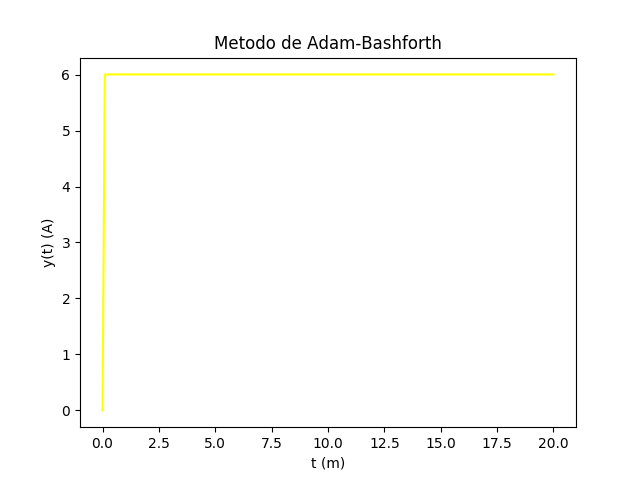
\includegraphics[width=.8\linewidth]{Images/q4/Adam_Bashforth_i1_q4.png}  
  \caption{Adam Bashforth}
\end{subfigure}
\begin{subfigure}{.5\textwidth}
  \centering
  % include second image
  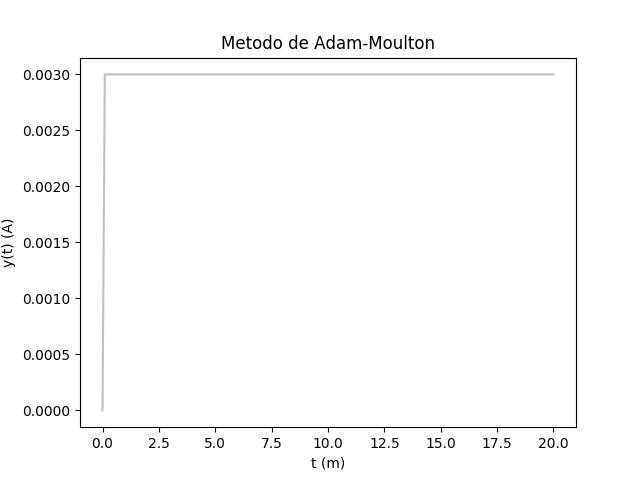
\includegraphics[width=.8\linewidth]{Images/q4/Adam_Moulton_i1_q4.png}  
  \caption{Adam Moulton}
\end{subfigure}

\newline

\begin{subfigure}{.5\textwidth}
  \centering
  % include third image
  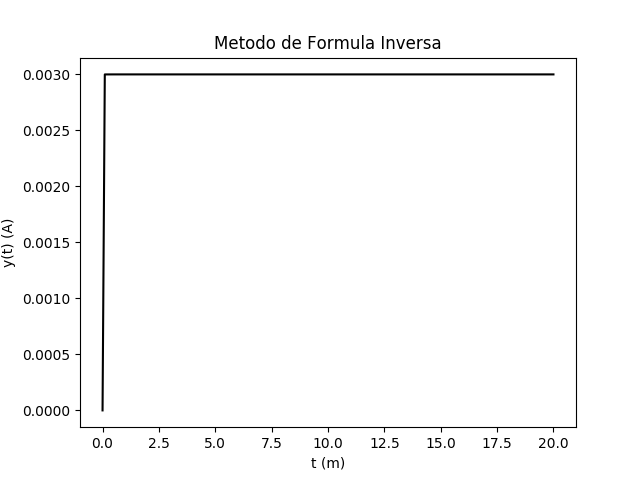
\includegraphics[width=.8\linewidth]{Images/q4/Formual_Inversa_i1_q4.png}  
  \caption{Formula Inversa}
\end{subfigure}
\caption{Métodos de Passos Múltiplos}
\end{figure}



\subsection{Gráfico da Solução Analítica}
O gráfico da solução exata para os valores das correntes $i_1$ e $i_2$ são mostradas na figura \ref{i:i1i2} abaixo

\begin{figure}[H]
\begin{subfigure}{.4\textwidth}
  \centering
  % include first image
  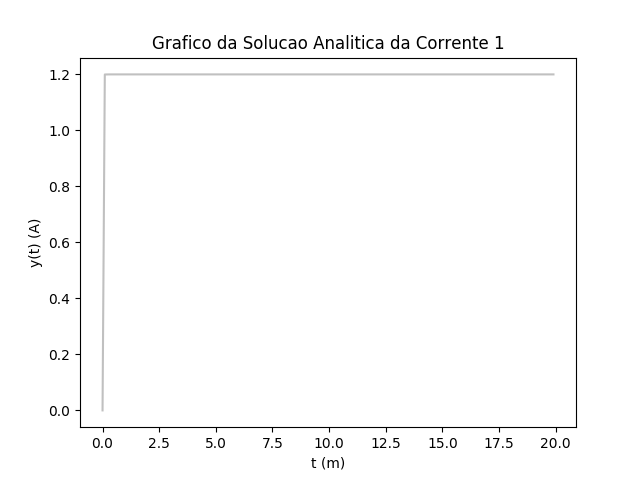
\includegraphics[width=.8\linewidth]{Images/Analytic_solve_i1_q4.png}
  \caption{Corrente $i_1$}
\end{subfigure}
\begin{subfigure}{.4\textwidth}
  \centering
  % include second image
  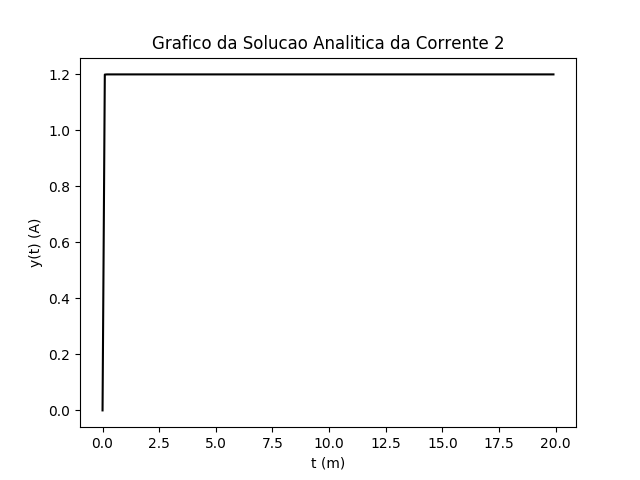
\includegraphics[width=.8\linewidth]{Images/Analytic_solve_i2_q4.png}
  \caption{Corrente $i_2$}
\end{subfigure}

\caption{gráficos das correntes $i_1$ e $i_2$}
\label{i:i1i2}
\end{figure}

\section{Conclusão}
Por meio desse projeto e com o que foi visto na disciplina, concluimos que, os métodos computacionais são essenciais para analisarmos funções diferenciais de tal modo que mesmo não conhecendo a função, conseguimos uma aproximação tão boa quanto.
\end{document}
